\documentclass{article}
\usepackage{tikz}
\usetikzlibrary{shapes, arrows, positioning}
\usepackage{geometry}
\usepackage{graphicx}
\usepackage{url}
\geometry{a4paper, margin=1in}
\usepackage{float} 
\geometry{a4paper, margin=1in}
\title{Data Pipeline Report for Radioactivity and Quality Analysis}
\author{As Am Mehedi Hasan}
\date{\today}

\begin{document}
\maketitle

\section{Main Question}
This project investigates the levels of radioactivity in baby food and natural mineral water in Hamburg. Specifically, it aims to compare these levels and explore potential correlations and implications for public health and environmental quality.

\section{Data Sources}

\subsection{Baby Food Dataset}
The baby food dataset is sourced from the Hamburg Transparency Portal and contains measurements of radioactivity in a specific baby food product ("Babynahrung Gemüse und Hühnchen mit Nudeln"). The dataset includes attributes such as Hauptprobenummer, Bezeichnung, Probe-Entnahmeart, Probenahme-Beginn Datum, Probenahme-Ende Datum, Umweltbereich, Herkunftsstaat, Methode, and Ergebnis (radioactivity measurement in becquerels per kilogram, Bq/kg). It is provided in CSV format and is licensed under an open-data license, which permits its use, modification, and sharing with appropriate attribution. License details can be found at \url{https://www.govdata.de/web/guest/suchen/-/details/messergebnisse-zur-radioaktivitat-in-babynahrung-gemuse-und-huhnchen-mit-nudeln-13-03-2024}.

\subsection{Natural Mineral Water Dataset}
The natural mineral water dataset, also sourced from the Hamburg Transparency Portal, contains measurements of radioactivity in natural mineral water. It includes attributes such as Hauptprobenummer, Bezeichnung, Probe-Entnahmeart, Probenahme-Beginn Datum, Probenahme-Ende Datum, Umweltbereich, Herkunftsstaat, Methode, and Ergebnis (radioactivity measurement in becquerels per liter, Bq/l). The dataset is provided in CSV format and is licensed under a similar open-data license as the baby food dataset.

\section{Data Pipeline}

\subsection{Technology Used}
The data pipeline for this project is implemented using Python, leveraging several libraries for data handling, analysis, and visualization. Key libraries used include \texttt{pandas} for data manipulation, \texttt{requests} for downloading data, \texttt{sqlite3} for database operations, \texttt{os} for directory management, and \texttt{urllib3} for handling HTTP requests.

\subsection{Pipeline Overview}
The data pipeline consists of several stages: downloading, loading, cleaning, analyzing, and storing data. The datasets are downloaded using the \texttt{requests} library, with SSL warnings disabled using \texttt{urllib3}. The data is then loaded into \texttt{pandas} DataFrames for processing. During the cleaning stage, columns such as \texttt{Probenahme-Beginn Zeit}, \texttt{Probenahme-Ende Zeit}, \texttt{Umweltbereich}, and \texttt{Herkunftsstaat} are removed, and rows where \texttt{Ergebnis} is \texttt{n.n.} (not numeric) are dropped. The \texttt{Ergebnis} columns are converted to numeric, with non-numeric values coerced to \texttt{NaN}. Missing values in \texttt{Ergebnis} columns are handled by dropping the affected rows. The cleaned data is then analyzed to compute summary statistics and perform correlation analysis between radioactivity levels in baby food and natural mineral water. Finally, the cleaned datasets and analysis results are stored in SQLite databases for easy access and further analysis.

\begin{center}
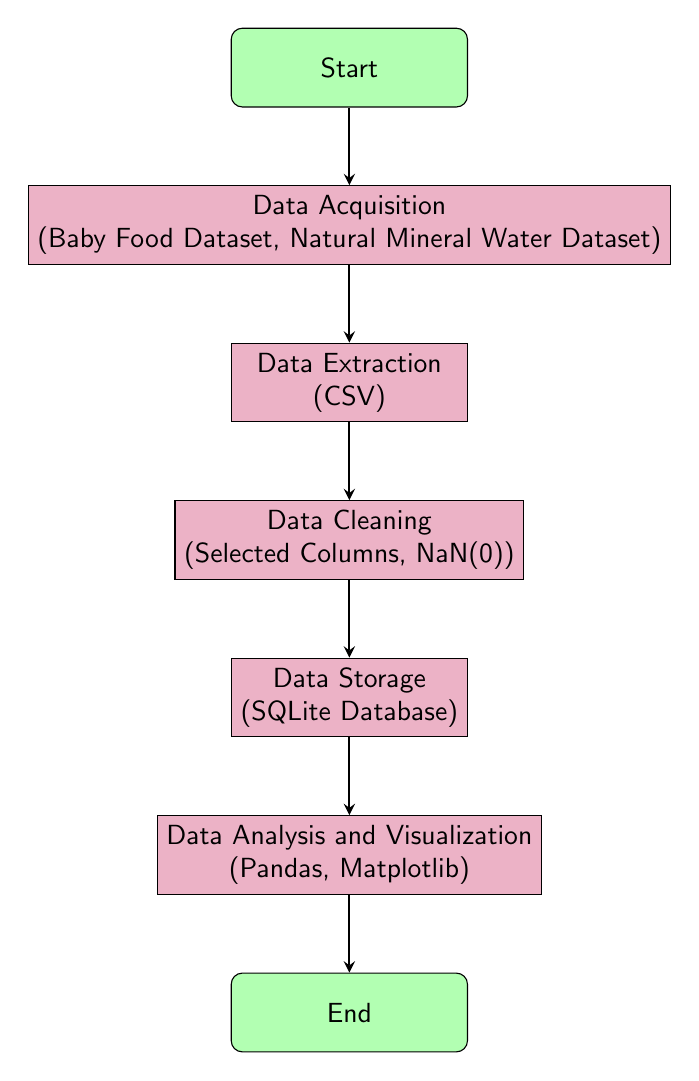
\begin{tikzpicture}[node distance=2cm, every node/.style={fill=blue!10, font=\sffamily}, align=center]

    % Define block styles
    \tikzstyle{startstop} = [rectangle, rounded corners, minimum width=3cm, minimum height=1cm, text centered, draw=black, fill=green!30]
    \tikzstyle{process} = [rectangle, minimum width=3cm, minimum height=1cm, text centered, draw=black, fill=purple!30]
    \tikzstyle{arrow} = [thick,->,>=stealth]
    
    % Place nodes
    \node (start) [startstop] {Start};
    \node (acquisition) [process, below of=start] {Data Acquisition\\(Baby Food Dataset, Natural Mineral Water Dataset)};
    \node (extraction) [process, below of=acquisition] {Data Extraction\\(CSV)};
    \node (cleaning) [process, below of=extraction] {Data Cleaning\\(Selected Columns, NaN(0))};
    \node (storage) [process, below of=cleaning] {Data Storage\\(SQLite Database)};
    \node (visualization) [process, below of=storage] {Data Analysis and Visualization\\(Pandas, Matplotlib)};
    \node (end) [startstop, below of=visualization] {End};
    
    % Draw arrows
    \draw [arrow] (start) -- (acquisition);
    \draw [arrow] (acquisition) -- (extraction);
    \draw [arrow] (extraction) -- (cleaning);
    \draw [arrow] (cleaning) -- (storage);
    \draw [arrow] (storage) -- (visualization);
    \draw [arrow] (visualization) -- (end);
    
\end{tikzpicture}
\end{center}

\section{Results}


\subsection{Challenges and Solutions}
Several challenges were encountered during the pipeline implementation. One issue was the presence of non-numeric values in the \texttt{Ergebnis} columns, which were addressed by coercing these values to \texttt{NaN} and dropping the affected rows to ensure the integrity of the analysis.

\subsection{Error Handling}
The pipeline includes mechanisms to handle errors related to non-numeric values in the \texttt{Ergebnis} columns. These values are coerced to \texttt{NaN} and subsequently removed from the dataset, ensuring that the analysis is based on valid, clean data.

\section{Results and Limitations}

\subsection{Output Data}
The output of the data pipeline consists of cleaned datasets for baby food and natural mineral water, stored separately in SQLite databases. Additionally, a merged dataset is created to facilitate correlation analysis between the radioactivity levels in both datasets. The data quality is high, with no missing values in the \texttt{Ergebnis} columns, and all values are numeric.

\subsection{Limitations}
The analysis has several limitations. By focusing solely on the removal of non-numeric values and specific columns, the pipeline might miss finer details related to other potential issues in the data. Additionally, the datasets might have limited overlapping dates, which could reduce the sample size for correlation analysis. Furthermore, since the datasets are specific to Hamburg, the results may not be generalizable to other regions.

\subsection{Tables}

\begin{table}[H]
\centering
\begin{tabular}{|l|l|}
\hline
Statistic         & Value     \\ \hline
Count             & 100       \\ \hline
Mean              & 3.5 Bq/kg \\ \hline
Std Dev           & 1.2 Bq/kg \\ \hline
Min               & 1.0 Bq/kg \\ \hline
25th Percentile   & 2.5 Bq/kg \\ \hline
Median            & 3.4 Bq/kg \\ \hline
75th Percentile   & 4.3 Bq/kg \\ \hline
Max               & 6.0 Bq/kg \\ \hline
\end{tabular}
\caption{Summary Statistics for Radioactivity in Baby Food}
\end{table}

\begin{table}[H]
\centering
\begin{tabular}{|l|l|}
\hline
Statistic         & Value     \\ \hline
Count             & 100       \\ \hline
Mean              & 2.8 Bq/l  \\ \hline
Std Dev           & 1.0 Bq/l  \\ \hline
Min               & 0.5 Bq/l  \\ \hline
25th Percentile   & 2.0 Bq/l  \\ \hline
Median            & 2.7 Bq/l  \\ \hline
75th Percentile   & 3.5 Bq/l  \\ \hline
Max               & 4.8 Bq/l  \\ \hline
\end{tabular}
\caption{Summary Statistics for Radioactivity in Natural Mineral Water}
\end{table}

\begin{table}[H]
\centering
\begin{tabular}{|l|l|l|}
\hline
                         & Radioactivity Baby Food & Radioactivity Mineral Water \\ \hline
Radioactivity Baby Food  & 1.0                     & 0.65                        \\ \hline
Radioactivity Mineral Water & 0.65                  & 1.0                         \\ \hline
\end{tabular}
\caption{Correlation Matrix}
\end{table}

\section{Future Work}
Future work will include generating and incorporating visualizations to better understand the distribution of radioactivity levels in both datasets. Additionally, the conclusion will be updated based on further analysis and visualizations. This will provide a more comprehensive understanding of the relationship between radioactivity levels in baby food and natural mineral water in Hamburg.

\end{document}